% REV00 Tue 04 May 2021 13:55:16 WIB
% START Tue 04 May 2021 13:55:16 WIB

\chapter{XXX}

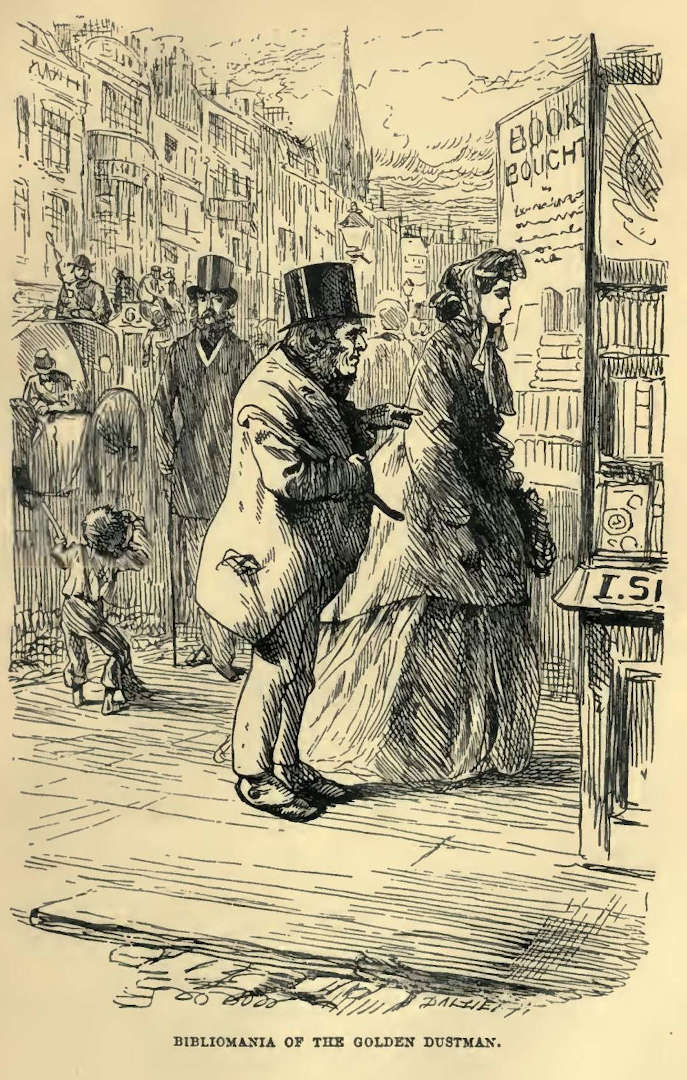
\includegraphics[scale=2.3]{03-05-01}

Chapter 10

SCOUTS OUT


‘And so, Miss Wren,’ said Mr Eugene Wrayburn, ‘I cannot persuade you to
dress me a doll?’

‘No,’ replied Miss Wren snappishly; ‘if you want one, go and buy one at
the shop.’

‘And my charming young goddaughter,’ said Mr Wrayburn plaintively, ‘down
in Hertfordshire--’

[‘Humbugshire you mean, I think,’ interposed Miss Wren.)

‘--is to be put upon the cold footing of the general public, and is
to derive no advantage from my private acquaintance with the Court
Dressmaker?’

‘If it’s any advantage to your charming godchild--and oh, a precious
godfather she has got!’--replied Miss Wren, pricking at him in the air
with her needle, ‘to be informed that the Court Dressmaker knows
your tricks and your manners, you may tell her so by post, with my
compliments.’

Miss Wren was busy at her work by candle-light, and Mr Wrayburn, half
amused and half vexed, and all idle and shiftless, stood by her bench
looking on. Miss Wren’s troublesome child was in the corner in deep
disgrace, and exhibiting great wretchedness in the shivering stage of
prostration from drink.

‘Ugh, you disgraceful boy!’ exclaimed Miss Wren, attracted by the sound
of his chattering teeth, ‘I wish they’d all drop down your throat and
play at dice in your stomach! Boh, wicked child! Bee-baa, black sheep!’

On her accompanying each of these reproaches with a threatening stamp of
the foot, the wretched creature protested with a whine.

‘Pay five shillings for you indeed!’ Miss Wren proceeded; ‘how many
hours do you suppose it costs me to earn five shillings, you infamous
boy?--Don’t cry like that, or I’ll throw a doll at you. Pay five
shillings fine for you indeed. Fine in more ways than one, I think! I’d
give the dustman five shillings, to carry you off in the dust cart.’

‘No, no,’ pleaded the absurd creature. ‘Please!’

‘He’s enough to break his mother’s heart, is this boy,’ said Miss Wren,
half appealing to Eugene. ‘I wish I had never brought him up. He’d be
sharper than a serpent’s tooth, if he wasn’t as dull as ditch water.
Look at him. There’s a pretty object for a parent’s eyes!’

Assuredly, in his worse than swinish state (for swine at least fatten on
their guzzling, and make themselves good to eat), he was a pretty object
for any eyes.

‘A muddling and a swipey old child,’ said Miss Wren, rating him with
great severity, ‘fit for nothing but to be preserved in the liquor
that destroys him, and put in a great glass bottle as a sight for other
swipey children of his own pattern,--if he has no consideration for his
liver, has he none for his mother?’

‘Yes. Deration, oh don’t!’ cried the subject of these angry remarks.

‘Oh don’t and oh don’t,’ pursued Miss Wren. ‘It’s oh do and oh do. And
why do you?’

‘Won’t do so any more. Won’t indeed. Pray!’

‘There!’ said Miss Wren, covering her eyes with her hand. ‘I can’t
bear to look at you. Go up stairs and get me my bonnet and shawl. Make
yourself useful in some way, bad boy, and let me have your room instead
of your company, for one half minute.’

Obeying her, he shambled out, and Eugene Wrayburn saw the tears exude
from between the little creature’s fingers as she kept her hand before
her eyes. He was sorry, but his sympathy did not move his carelessness
to do anything but feel sorry.

‘I’m going to the Italian Opera to try on,’ said Miss Wren, taking away
her hand after a little while, and laughing satirically to hide that she
had been crying; ‘I must see your back before I go, Mr Wrayburn. Let me
first tell you, once for all, that it’s of no use your paying visits
to me. You wouldn’t get what you want, of me, no, not if you brought
pincers with you to tear it out.’

‘Are you so obstinate on the subject of a doll’s dress for my godchild?’

‘Ah!’ returned Miss Wren with a hitch of her chin, ‘I am so
obstinate. And of course it’s on the subject of a doll’s dress--or
ADdress--whichever you like. Get along and give it up!’

Her degraded charge had come back, and was standing behind her with the
bonnet and shawl.

‘Give ‘em to me and get back into your corner, you naughty old thing!’
said Miss Wren, as she turned and espied him. ‘No, no, I won’t have your
help. Go into your corner, this minute!’

The miserable man, feebly rubbing the back of his faltering hands
downward from the wrists, shuffled on to his post of disgrace; but not
without a curious glance at Eugene in passing him, accompanied with what
seemed as if it might have been an action of his elbow, if any action of
any limb or joint he had, would have answered truly to his will. Taking
no more particular notice of him than instinctively falling away from
the disagreeable contact, Eugene, with a lazy compliment or so to Miss
Wren, begged leave to light his cigar, and departed.

‘Now you prodigal old son,’ said Jenny, shaking her head and her
emphatic little forefinger at her burden, ‘you sit there till I come
back. You dare to move out of your corner for a single instant while I’m
gone, and I’ll know the reason why.’

With this admonition, she blew her work candles out, leaving him to the
light of the fire, and, taking her big door-key in her pocket and her
crutch-stick in her hand, marched off.

Eugene lounged slowly towards the Temple, smoking his cigar, but saw
no more of the dolls’ dressmaker, through the accident of their taking
opposite sides of the street. He lounged along moodily, and stopped at
Charing Cross to look about him, with as little interest in the crowd
as any man might take, and was lounging on again, when a most unexpected
object caught his eyes. No less an object than Jenny Wren’s bad boy
trying to make up his mind to cross the road.

A more ridiculous and feeble spectacle than this tottering wretch making
unsteady sallies into the roadway, and as often staggering back again,
oppressed by terrors of vehicles that were a long way off or were
nowhere, the streets could not have shown. Over and over again, when the
course was perfectly clear, he set out, got half way, described a loop,
turned, and went back again; when he might have crossed and re-crossed
half a dozen times. Then, he would stand shivering on the edge of the
pavement, looking up the street and looking down, while scores of people
jostled him, and crossed, and went on. Stimulated in course of time
by the sight of so many successes, he would make another sally, make
another loop, would all but have his foot on the opposite pavement,
would see or imagine something coming, and would stagger back again.
There, he would stand making spasmodic preparations as if for a great
leap, and at last would decide on a start at precisely the wrong moment,
and would be roared at by drivers, and would shrink back once more, and
stand in the old spot shivering, with the whole of the proceedings to go
through again.

‘It strikes me,’ remarked Eugene coolly, after watching him for some
minutes, ‘that my friend is likely to be rather behind time if he has
any appointment on hand.’ With which remark he strolled on, and took no
further thought of him.

Lightwood was at home when he got to the Chambers, and had dined alone
there. Eugene drew a chair to the fire by which he was having his wine
and reading the evening paper, and brought a glass, and filled it for
good fellowship’s sake.

‘My dear Mortimer, you are the express picture of contented industry,
reposing (on credit) after the virtuous labours of the day.’

‘My dear Eugene, you are the express picture of discontented idleness
not reposing at all. Where have you been?’

‘I have been,’ replied Wrayburn, ‘--about town. I have turned up at the
present juncture, with the intention of consulting my highly intelligent
and respected solicitor on the position of my affairs.’

‘Your highly intelligent and respect solicitor is of opinion that your
affairs are in a bad way, Eugene.’

‘Though whether,’ said Eugene thoughtfully, ‘that can be intelligently
said, now, of the affairs of a client who has nothing to lose and who
cannot possibly be made to pay, may be open to question.’

‘You have fallen into the hands of the Jews, Eugene.’

‘My dear boy,’ returned the debtor, very composedly taking up his glass,
‘having previously fallen into the hands of some of the Christians, I
can bear it with philosophy.’

‘I have had an interview to-day, Eugene, with a Jew, who seems
determined to press us hard. Quite a Shylock, and quite a Patriarch. A
picturesque grey-headed and grey-bearded old Jew, in a shovel-hat and
gaberdine.’

‘Not,’ said Eugene, pausing in setting down his glass, ‘surely not my
worthy friend Mr Aaron?’

‘He calls himself Mr Riah.’

‘By-the-by,’ said Eugene, ‘it comes into my mind that--no doubt with an
instinctive desire to receive him into the bosom of our Church--I gave
him the name of Aaron!’

‘Eugene, Eugene,’ returned Lightwood, ‘you are more ridiculous than
usual. Say what you mean.’

‘Merely, my dear fellow, that I have the honour and pleasure of a
speaking acquaintance with such a Patriarch as you describe, and that I
address him as Mr Aaron, because it appears to me Hebraic, expressive,
appropriate, and complimentary. Notwithstanding which strong reasons for
its being his name, it may not be his name.’

‘I believe you are the absurdest man on the face of the earth,’ said
Lightwood, laughing.

‘Not at all, I assure you. Did he mention that he knew me?’

‘He did not. He only said of you that he expected to be paid by you.’

‘Which looks,’ remarked Eugene with much gravity, ‘like NOT knowing me.
I hope it may not be my worthy friend Mr Aaron, for, to tell you the
truth, Mortimer, I doubt he may have a prepossession against me. I
strongly suspect him of having had a hand in spiriting away Lizzie.’

‘Everything,’ returned Lightwood impatiently, ‘seems, by a fatality,
to bring us round to Lizzie. “About town” meant about Lizzie, just now,
Eugene.’

‘My solicitor, do you know,’ observed Eugene, turning round to the
furniture, ‘is a man of infinite discernment!’

‘Did it not, Eugene?’

‘Yes it did, Mortimer.’

‘And yet, Eugene, you know you do not really care for her.’

Eugene Wrayburn rose, and put his hands in his pockets, and stood with a
foot on the fender, indolently rocking his body and looking at the fire.
After a prolonged pause, he replied: ‘I don’t know that. I must ask you
not to say that, as if we took it for granted.’

‘But if you do care for her, so much the more should you leave her to
herself.’

Having again paused as before, Eugene said: ‘I don’t know that, either.
But tell me. Did you ever see me take so much trouble about anything, as
about this disappearance of hers? I ask, for information.’

‘My dear Eugene, I wish I ever had!’

‘Then you have not? Just so. You confirm my own impression. Does that
look as if I cared for her? I ask, for information.’

‘I asked YOU for information, Eugene,’ said Mortimer reproachfully.

‘Dear boy, I know it, but I can’t give it. I thirst for information.
What do I mean? If my taking so much trouble to recover her does not
mean that I care for her, what does it mean? “If Peter Piper picked a
peck of pickled pepper, where’s the peck,” \& c.?’

Though he said this gaily, he said it with a perplexed and inquisitive
face, as if he actually did not know what to make of himself. ‘Look on
to the end--’ Lightwood was beginning to remonstrate, when he caught at
the words:

‘Ah! See now! That’s exactly what I am incapable of doing. How very
acute you are, Mortimer, in finding my weak place! When we were at
school together, I got up my lessons at the last moment, day by day and
bit by bit; now we are out in life together, I get up my lessons in the
same way. In the present task I have not got beyond this:--I am bent
on finding Lizzie, and I mean to find her, and I will take any means
of finding her that offer themselves. Fair means or foul means, are all
alike to me. I ask you--for information--what does that mean? When I
have found her I may ask you--also for information--what do I mean now?
But it would be premature in this stage, and it’s not the character of
my mind.’

Lightwood was shaking his head over the air with which his friend held
forth thus--an air so whimsically open and argumentative as almost to
deprive what he said of the appearance of evasion--when a shuffling was
heard at the outer door, and then an undecided knock, as though
some hand were groping for the knocker. ‘The frolicsome youth of the
neighbourhood,’ said Eugene, ‘whom I should be delighted to pitch from
this elevation into the churchyard below, without any intermediate
ceremonies, have probably turned the lamp out. I am on duty to-night,
and will see to the door.’

His friend had barely had time to recall the unprecedented gleam of
determination with which he had spoken of finding this girl, and which
had faded out of him with the breath of the spoken words, when Eugene
came back, ushering in a most disgraceful shadow of a man, shaking from
head to foot, and clothed in shabby grease and smear.

‘This interesting gentleman,’ said Eugene, ‘is the son--the
occasionally rather trying son, for he has his failings--of a lady of my
acquaintance. My dear Mortimer--Mr Dolls.’ Eugene had no idea what his
name was, knowing the little dressmaker’s to be assumed, but presented
him with easy confidence under the first appellation that his
associations suggested.

‘I gather, my dear Mortimer,’ pursued Eugene, as Lightwood stared at
the obscene visitor, ‘from the manner of Mr Dolls--which is occasionally
complicated--that he desires to make some communication to me. I have
mentioned to Mr Dolls that you and I are on terms of confidence, and
have requested Mr Dolls to develop his views here.’

The wretched object being much embarrassed by holding what remained
of his hat, Eugene airily tossed it to the door, and put him down in a
chair.

‘It will be necessary, I think,’ he observed, ‘to wind up Mr Dolls,
before anything to any mortal purpose can be got out of him. Brandy, Mr
Dolls, or--?’

‘Threepenn’orth Rum,’ said Mr Dolls.

A judiciously small quantity of the spirit was given him in a
wine-glass, and he began to convey it to his mouth, with all kinds of
falterings and gyrations on the road.

‘The nerves of Mr Dolls,’ remarked Eugene to Lightwood, ‘are
considerably unstrung. And I deem it on the whole expedient to fumigate
Mr Dolls.’

He took the shovel from the grate, sprinkled a few live ashes on it, and
from a box on the chimney-piece took a few pastiles, which he set upon
them; then, with great composure began placidly waving the shovel in
front of Mr Dolls, to cut him off from his company.

‘Lord bless my soul, Eugene!’ cried Lightwood, laughing again, ‘what a
mad fellow you are! Why does this creature come to see you?’

‘We shall hear,’ said Wrayburn, very observant of his face withal. ‘Now
then. Speak out. Don’t be afraid. State your business, Dolls.’

‘Mist Wrayburn!’ said the visitor, thickly and huskily. ‘--‘TIS Mist
Wrayburn, ain’t?’ With a stupid stare.

‘Of course it is. Look at me. What do you want?’

Mr Dolls collapsed in his chair, and faintly said ‘Threepenn’orth Rum.’

‘Will you do me the favour, my dear Mortimer, to wind up Mr Dolls
again?’ said Eugene. ‘I am occupied with the fumigation.’

A similar quantity was poured into his glass, and he got it to his lips
by similar circuitous ways. Having drunk it, Mr Dolls, with an evident
fear of running down again unless he made haste, proceeded to business.

‘Mist Wrayburn. Tried to nudge you, but you wouldn’t. You want that
drection. You want t’know where she lives. DO you Mist Wrayburn?’

With a glance at his friend, Eugene replied to the question sternly, ‘I
do.’

‘I am er man,’ said Mr Dolls, trying to smite himself on the breast, but
bringing his hand to bear upon the vicinity of his eye, ‘er do it. I am
er man er do it.’

‘What are you the man to do?’ demanded Eugene, still sternly.

‘Er give up that drection.’

‘Have you got it?’

With a most laborious attempt at pride and dignity, Mr Dolls rolled
his head for some time, awakening the highest expectations, and then
answered, as if it were the happiest point that could possibly be
expected of him: ‘No.’

‘What do you mean then?’

Mr Dolls, collapsing in the drowsiest manner after his late intellectual
triumph, replied: ‘Threepenn’orth Rum.’

‘Wind him up again, my dear Mortimer,’ said Wrayburn; ‘wind him up
again.’

‘Eugene, Eugene,’ urged Lightwood in a low voice, as he complied, ‘can
you stoop to the use of such an instrument as this?’

‘I said,’ was the reply, made with that former gleam of determination,
‘that I would find her out by any means, fair or foul. These are foul,
and I’ll take them--if I am not first tempted to break the head of Mr
Dolls with the fumigator. Can you get the direction? Do you mean that?
Speak! If that’s what you have come for, say how much you want.’

‘Ten shillings--Threepenn’orths Rum,’ said Mr Dolls.

‘You shall have it.’

‘Fifteen shillings--Threepenn’orths Rum,’ said Mr Dolls, making an
attempt to stiffen himself.

‘You shall have it. Stop at that. How will you get the direction you
talk of?’

‘I am er man,’ said Mr Dolls, with majesty, ‘er get it, sir.’

‘How will you get it, I ask you?’

‘I am ill-used vidual,’ said Mr Dolls. ‘Blown up morning t’night. Called
names. She makes Mint money, sir, and never stands Threepenn’orth Rum.’

‘Get on,’ rejoined Eugene, tapping his palsied head with the
fire-shovel, as it sank on his breast. ‘What comes next?’

Making a dignified attempt to gather himself together, but, as it were,
dropping half a dozen pieces of himself while he tried in vain to pick
up one, Mr Dolls, swaying his head from side to side, regarded his
questioner with what he supposed to be a haughty smile and a scornful
glance.

‘She looks upon me as mere child, sir. I am NOT mere child, sir. Man.
Man talent. Lerrers pass betwixt ‘em. Postman lerrers. Easy for man
talent er get drection, as get his own drection.’

‘Get it then,’ said Eugene; adding very heartily under his breath,
‘--You Brute! Get it, and bring it here to me, and earn the money for
sixty threepenn’orths of rum, and drink them all, one a top of another,
and drink yourself dead with all possible expedition.’ The latter
clauses of these special instructions he addressed to the fire, as he
gave it back the ashes he had taken from it, and replaced the shovel.

Mr Dolls now struck out the highly unexpected discovery that he had been
insulted by Lightwood, and stated his desire to ‘have it out with him’
on the spot, and defied him to come on, upon the liberal terms of
a sovereign to a halfpenny. Mr Dolls then fell a crying, and then
exhibited a tendency to fall asleep. This last manifestation as by far
the most alarming, by reason of its threatening his prolonged stay
on the premises, necessitated vigorous measures. Eugene picked up his
worn-out hat with the tongs, clapped it on his head, and, taking him by
the collar--all this at arm’s length--conducted him down stairs and out
of the precincts into Fleet Street. There, he turned his face westward,
and left him.

When he got back, Lightwood was standing over the fire, brooding in a
sufficiently low-spirited manner.

‘I’ll wash my hands of Mr Dolls physically--’ said Eugene, ‘and be with
you again directly, Mortimer.’

‘I would much prefer,’ retorted Mortimer, ‘your washing your hands of Mr
Dolls, morally, Eugene.’

‘So would I,’ said Eugene; ‘but you see, dear boy, I can’t do without
him.’

In a minute or two he resumed his chair, as perfectly unconcerned as
usual, and rallied his friend on having so narrowly escaped the prowess
of their muscular visitor.

‘I can’t be amused on this theme,’ said Mortimer, restlessly. ‘You can
make almost any theme amusing to me, Eugene, but not this.’

‘Well!’ cried Eugene, ‘I am a little ashamed of it myself, and therefore
let us change the subject.’

‘It is so deplorably underhanded,’ said Mortimer. ‘It is so unworthy of
you, this setting on of such a shameful scout.’

‘We have changed the subject!’ exclaimed Eugene, airily. ‘We have found
a new one in that word, scout. Don’t be like Patience on a mantelpiece
frowning at Dolls, but sit down, and I’ll tell you something that you
really will find amusing. Take a cigar. Look at this of mine. I
light it--draw one puff--breathe the smoke out--there it goes--it’s
Dolls!--it’s gone--and being gone you are a man again.’

‘Your subject,’ said Mortimer, after lighting a cigar, and comforting
himself with a whiff or two, ‘was scouts, Eugene.’

‘Exactly. Isn’t it droll that I never go out after dark, but I find
myself attended, always by one scout, and often by two?’

Lightwood took his cigar from his lips in surprise, and looked at his
friend, as if with a latent suspicion that there must be a jest or
hidden meaning in his words.

‘On my honour, no,’ said Wrayburn, answering the look and smiling
carelessly; ‘I don’t wonder at your supposing so, but on my honour, no.
I say what I mean. I never go out after dark, but I find myself in the
ludicrous situation of being followed and observed at a distance, always
by one scout, and often by two.’

‘Are you sure, Eugene?’

‘Sure? My dear boy, they are always the same.’

‘But there’s no process out against you. The Jews only threaten. They
have done nothing. Besides, they know where to find you, and I represent
you. Why take the trouble?’

‘Observe the legal mind!’ remarked Eugene, turning round to the
furniture again, with an air of indolent rapture. ‘Observe the dyer’s
hand, assimilating itself to what it works in,--or would work in, if
anybody would give it anything to do. Respected solicitor, it’s not
that. The schoolmaster’s abroad.’

‘The schoolmaster?’

‘Ay! Sometimes the schoolmaster and the pupil are both abroad. Why, how
soon you rust in my absence! You don’t understand yet? Those fellows
who were here one night. They are the scouts I speak of, as doing me the
honour to attend me after dark.’

‘How long has this been going on?’ asked Lightwood, opposing a serious
face to the laugh of his friend.

‘I apprehend it has been going on, ever since a certain person went off.
Probably, it had been going on some little time before I noticed it:
which would bring it to about that time.’

‘Do you think they suppose you to have inveigled her away?’

‘My dear Mortimer, you know the absorbing nature of my professional
occupations; I really have not had leisure to think about it.’

‘Have you asked them what they want? Have you objected?’

‘Why should I ask them what they want, dear fellow, when I am
indifferent what they want? Why should I express objection, when I don’t
object?’

‘You are in your most reckless mood. But you called the situation just
now, a ludicrous one; and most men object to that, even those who are
utterly indifferent to everything else.’

‘You charm me, Mortimer, with your reading of my weaknesses. (By-the-by,
that very word, Reading, in its critical use, always charms me. An
actress’s Reading of a chambermaid, a dancer’s Reading of a hornpipe, a
singer’s Reading of a song, a marine painter’s Reading of the sea,
the kettle-drum’s Reading of an instrumental passage, are phrases
ever youthful and delightful.) I was mentioning your perception of my
weaknesses. I own to the weakness of objecting to occupy a ludicrous
position, and therefore I transfer the position to the scouts.’

‘I wish, Eugene, you would speak a little more soberly and plainly, if
it were only out of consideration for my feeling less at ease than you
do.’

‘Then soberly and plainly, Mortimer, I goad the schoolmaster to madness.
I make the schoolmaster so ridiculous, and so aware of being made
ridiculous, that I see him chafe and fret at every pore when we cross
one another. The amiable occupation has been the solace of my life,
since I was baulked in the manner unnecessary to recall. I have derived
inexpressible comfort from it. I do it thus: I stroll out after dark,
stroll a little way, look in at a window and furtively look out for the
schoolmaster. Sooner or later, I perceive the schoolmaster on the watch;
sometimes accompanied by his hopeful pupil; oftener, pupil-less. Having
made sure of his watching me, I tempt him on, all over London. One
night I go east, another night north, in a few nights I go all round the
compass. Sometimes, I walk; sometimes, I proceed in cabs, draining the
pocket of the schoolmaster who then follows in cabs. I study and get
up abstruse No Thoroughfares in the course of the day. With Venetian
mystery I seek those No Thoroughfares at night, glide into them by means
of dark courts, tempt the schoolmaster to follow, turn suddenly, and
catch him before he can retreat. Then we face one another, and I pass
him as unaware of his existence, and he undergoes grinding torments.
Similarly, I walk at a great pace down a short street, rapidly turn the
corner, and, getting out of his view, as rapidly turn back. I catch him
coming on post, again pass him as unaware of his existence, and again
he undergoes grinding torments. Night after night his disappointment is
acute, but hope springs eternal in the scholastic breast, and he follows
me again to-morrow. Thus I enjoy the pleasures of the chase, and derive
great benefit from the healthful exercise. When I do not enjoy the
pleasures of the chase, for anything I know he watches at the Temple
Gate all night.’

‘This is an extraordinary story,’ observed Lightwood, who had heard it
out with serious attention. ‘I don’t like it.’

‘You are a little hipped, dear fellow,’ said Eugene; ‘you have been too
sedentary. Come and enjoy the pleasures of the chase.’

‘Do you mean that you believe he is watching now?’

‘I have not the slightest doubt he is.’

‘Have you seen him to-night?’

‘I forgot to look for him when I was last out,’ returned Eugene with the
calmest indifference; ‘but I dare say he was there. Come! Be a British
sportsman and enjoy the pleasures of the chase. It will do you good.’

Lightwood hesitated; but, yielding to his curiosity, rose.

‘Bravo!’ cried Eugene, rising too. ‘Or, if Yoicks would be in better
keeping, consider that I said Yoicks. Look to your feet, Mortimer, for
we shall try your boots. When you are ready, I am--need I say with a Hey
Ho Chivey, and likewise with a Hark Forward, Hark Forward, Tantivy?’

‘Will nothing make you serious?’ said Mortimer, laughing through his
gravity.

‘I am always serious, but just now I am a little excited by the glorious
fact that a southerly wind and a cloudy sky proclaim a hunting evening.
Ready? So. We turn out the lamp and shut the door, and take the field.’

As the two friends passed out of the Temple into the public street,
Eugene demanded with a show of courteous patronage in which direction
Mortimer would you like the run to be? ‘There is a rather difficult
country about Bethnal Green,’ said Eugene, ‘and we have not taken in
that direction lately. What is your opinion of Bethnal Green?’ Mortimer
assented to Bethnal Green, and they turned eastward. ‘Now, when we come
to St Paul’s churchyard,’ pursued Eugene, ‘we’ll loiter artfully, and
I’ll show you the schoolmaster.’ But, they both saw him, before they got
there; alone, and stealing after them in the shadow of the houses, on
the opposite side of the way.

‘Get your wind,’ said Eugene, ‘for I am off directly. Does it occur
to you that the boys of Merry England will begin to deteriorate in an
educational light, if this lasts long? The schoolmaster can’t attend to
me and the boys too. Got your wind? I am off!’

At what a rate he went, to breathe the schoolmaster; and how he then
lounged and loitered, to put his patience to another kind of wear;
what preposterous ways he took, with no other object on earth than to
disappoint and punish him; and how he wore him out by every piece of
ingenuity that his eccentric humour could devise; all this Lightwood
noted, with a feeling of astonishment that so careless a man could be so
wary, and that so idle a man could take so much trouble. At last, far on
in the third hour of the pleasures of the chase, when he had brought the
poor dogging wretch round again into the City, he twisted Mortimer up
a few dark entries, twisted him into a little square court, twisted him
sharp round again, and they almost ran against Bradley Headstone.

‘And you see, as I was saying, Mortimer,’ remarked Eugene aloud with
the utmost coolness, as though there were no one within hearing
by themselves: ‘and you see, as I was saying--undergoing grinding
torments.’

It was not too strong a phrase for the occasion. Looking like the hunted
and not the hunter, baffled, worn, with the exhaustion of deferred
hope and consuming hate and anger in his face, white-lipped, wild-eyed,
draggle-haired, seamed with jealousy and anger, and torturing himself
with the conviction that he showed it all and they exulted in it, he
went by them in the dark, like a haggard head suspended in the air: so
completely did the force of his expression cancel his figure.

Mortimer Lightwood was not an extraordinarily impressible man, but this
face impressed him. He spoke of it more than once on the remainder of
the way home, and more than once when they got home.

They had been abed in their respective rooms two or three hours, when
Eugene was partly awakened by hearing a footstep going about, and was
fully awakened by seeing Lightwood standing at his bedside.

‘Nothing wrong, Mortimer?’

‘No.’

‘What fancy takes you, then, for walking about in the night?’

‘I am horribly wakeful.’

‘How comes that about, I wonder!’

‘Eugene, I cannot lose sight of that fellow’s face.’

‘Odd!’ said Eugene with a light laugh, ‘I can.’ And turned over, and
fell asleep again.



